% Part 3: Basic Usage - Agentic Coding Tools
% LaTeX Beamer Presentation
% University of South Carolina Branding

\documentclass[aspectratio=169,11pt]{beamer}

% ============================================================
% THEME AND COLOR SETUP
% ============================================================
\usetheme{Madrid}
\usecolortheme{default}

% Remove rounded corners - sharp edges only
\setbeamertemplate{blocks}[default]
\setbeamertemplate{title page}[default][colsep=-4bp,rounded=false]
\setbeamertemplate{frametitle}[default][colsep=-4bp,rounded=false]

% UofSC Color Palette
\definecolor{UofSCGarnet}{HTML}{73000a}
\definecolor{UofSCBlack}{HTML}{000000}
\definecolor{UofSCWhite}{HTML}{ffffff}
\definecolor{UofSCRose}{HTML}{CC2E40}
\definecolor{UofSCAtlantic}{HTML}{466A9F}
\definecolor{UofSCCongaree}{HTML}{1F414D}
\definecolor{UofSCHorseshoe}{HTML}{65780B}
\definecolor{UofSCGrass}{HTML}{CED318}
\definecolor{UofSCHoneycomb}{HTML}{A49137}
\definecolor{UofSC90Black}{HTML}{363636}
\definecolor{UofSC70Black}{HTML}{5C5C5C}
\definecolor{UofSC50Black}{HTML}{A2A2A2}
\definecolor{UofSCWarmGrey}{HTML}{676156}
\definecolor{UofSCSandstorm}{HTML}{FFF2E3}
\definecolor{UofSCDarkGarnet}{HTML}{570008}
\definecolor{UofSCAzalea}{HTML}{844247}

% Apply UofSC colors to Beamer elements
\setbeamercolor{palette primary}{bg=UofSCGarnet,fg=UofSCWhite}
\setbeamercolor{palette secondary}{bg=UofSCCongaree,fg=UofSCWhite}
\setbeamercolor{palette tertiary}{bg=UofSCAtlantic,fg=UofSCWhite}
\setbeamercolor{palette quaternary}{bg=UofSCBlack,fg=UofSCWhite}
\setbeamercolor{structure}{fg=UofSCGarnet}
\setbeamercolor{section in toc}{fg=UofSCBlack}
\setbeamercolor{subsection in toc}{fg=UofSCGarnet}
\setbeamercolor{title}{fg=UofSCWhite,bg=UofSCGarnet}
\setbeamercolor{frametitle}{fg=UofSCWhite,bg=UofSCGarnet}
\setbeamercolor{block title}{bg=UofSCGarnet,fg=UofSCWhite}
\setbeamercolor{block body}{bg=UofSCSandstorm,fg=UofSCBlack}
\setbeamercolor{block title alerted}{bg=UofSCRose,fg=UofSCWhite}
\setbeamercolor{block body alerted}{bg=UofSCSandstorm,fg=UofSCBlack}
\setbeamercolor{block title example}{bg=UofSCAtlantic,fg=UofSCWhite}
\setbeamercolor{block body example}{bg=UofSCSandstorm,fg=UofSCBlack}
\setbeamercolor{itemize item}{fg=UofSCGarnet}
\setbeamercolor{itemize subitem}{fg=UofSCAtlantic}
\setbeamercolor{enumerate item}{fg=UofSCGarnet}
\setbeamercolor{description item}{fg=UofSCGarnet}
\setbeamercolor{caption name}{fg=UofSCGarnet}
\setbeamercolor{footnote}{fg=UofSC70Black}
\setbeamercolor{footnote mark}{fg=UofSCGarnet}

% Sharp itemize bullets
\setbeamertemplate{itemize item}{\tiny$\blacksquare$}
\setbeamertemplate{itemize subitem}{\tiny$\blacktriangleright$}
\setbeamertemplate{itemize subsubitem}{\tiny$\bullet$}

% Navigation symbols off
\setbeamertemplate{navigation symbols}{}

% Footer with slide numbers
\setbeamertemplate{footline}{
  \leavevmode%
  \hbox{%
  \begin{beamercolorbox}[wd=.333333\paperwidth,ht=2.25ex,dp=1ex,center]{author in head/foot}%
    \usebeamerfont{author in head/foot}\insertshortauthor
  \end{beamercolorbox}%
  \begin{beamercolorbox}[wd=.333333\paperwidth,ht=2.25ex,dp=1ex,center]{title in head/foot}%
    \usebeamerfont{title in head/foot}\insertshorttitle
  \end{beamercolorbox}%
  \begin{beamercolorbox}[wd=.333333\paperwidth,ht=2.25ex,dp=1ex,right]{date in head/foot}%
    \usebeamerfont{date in head/foot}\insertshortdate{}\hspace*{2em}
    \insertframenumber{} / \inserttotalframenumber\hspace*{2ex}
  \end{beamercolorbox}}%
  \vskip0pt%
}

% ============================================================
% PACKAGES
% ============================================================
\usepackage[utf8]{inputenc}
\usepackage[T1]{fontenc}
\usepackage{lmodern}
\usepackage{graphicx}
\usepackage{tikz}
\usetikzlibrary{shapes.geometric,arrows.meta,positioning,calc,fit,backgrounds,decorations.pathreplacing}
\usepackage{listings}
\usepackage{xcolor}
\usepackage{booktabs}
\usepackage{hyperref}
\usepackage{fontawesome5}

% ============================================================
% CODE LISTINGS SETUP
% ============================================================
\lstset{
    basicstyle=\ttfamily\scriptsize,
    keywordstyle=\color{UofSCGarnet}\bfseries,
    commentstyle=\color{UofSC70Black}\itshape,
    stringstyle=\color{UofSCAtlantic},
    numbers=left,
    numberstyle=\tiny\color{UofSC50Black},
    stepnumber=1,
    numbersep=5pt,
    backgroundcolor=\color{UofSCSandstorm},
    showspaces=false,
    showstringspaces=false,
    showtabs=false,
    frame=single,
    rulecolor=\color{UofSC70Black},
    tabsize=2,
    captionpos=b,
    breaklines=true,
    breakatwhitespace=false,
    escapeinside={(*@}{@*)},
    morekeywords={aider,claude,gh,copilot},
    xleftmargin=0.5cm,
    xrightmargin=0.5cm
}

\lstdefinelanguage{bash}{
    keywords={aider,claude,code,gh,copilot,suggest,explain,git,commit,push,pull,merge,branch,pip,install,pytest,python,curl},
    sensitive=true,
    morecomment=[l]{\#},
    morestring=[b]",
    morestring=[b]'
}

\lstdefinelanguage{python}{
    keywords={def,class,return,if,else,elif,for,while,import,from,as,try,except,raise,with,async,await,None,True,False,and,or,not,in,is,lambda},
    sensitive=true,
    morecomment=[l]{\#},
    morestring=[b]",
    morestring=[b]'
}

% ============================================================
% TIKZ STYLES
% ============================================================
\tikzset{
    % Sharp-cornered boxes
    process/.style={
        rectangle,
        draw=UofSCBlack,
        thick,
        fill=UofSCWhite,
        text=UofSCBlack,
        minimum width=3cm,
        minimum height=0.8cm,
        align=center,
        font=\small
    },
    process highlight/.style={
        process,
        fill=UofSCGarnet,
        text=UofSCWhite
    },
    process secondary/.style={
        process,
        fill=UofSCAtlantic,
        text=UofSCWhite
    },
    process tertiary/.style={
        process,
        fill=UofSCCongaree,
        text=UofSCWhite
    },
    arrow/.style={
        ->,
        >=Stealth,
        thick,
        color=UofSCBlack
    },
    arrow garnet/.style={
        arrow,
        color=UofSCGarnet
    },
    label box/.style={
        rectangle,
        draw=none,
        fill=UofSCSandstorm,
        text=UofSCBlack,
        font=\scriptsize,
        align=center
    },
    decision/.style={
        diamond,
        draw=UofSCBlack,
        thick,
        fill=UofSCHoneycomb,
        text=UofSCBlack,
        minimum width=2cm,
        minimum height=1cm,
        align=center,
        font=\small,
        aspect=2
    }
}

% ============================================================
% TITLE INFORMATION
% ============================================================
\title[Part 3: Basic Usage]{Part 3: Basic Usage}
\subtitle{Agentic Coding Tools -- A Comprehensive Guide}
\author[J. Vaught]{Instructor Name}
\institute[UofSC]{
    University of South Carolina\\
    \vspace{0.3cm}
    \includegraphics[height=1cm]{example-image}% Replace with UofSC logo
}
\date{\today}

% ============================================================
% DOCUMENT BEGIN
% ============================================================
\begin{document}

% Title Frame
\begin{frame}[plain]
    \titlepage
\end{frame}

% Table of Contents
\begin{frame}{Table of Contents}
    \tableofcontents
\end{frame}

% ============================================================
% SECTION 1: CORE CAPABILITIES OVERVIEW
% ============================================================
\section{Core Capabilities Overview}

\begin{frame}{What Are Agentic Coding Tools?}
    \begin{columns}[T]
        \begin{column}{0.55\textwidth}
            \textbf{AI-powered assistants} that understand and interact with your development environment autonomously.

            \vspace{0.3cm}
            Unlike traditional code completion, these tools:
            \begin{itemize}
                \item Execute terminal commands directly
                \item Read and modify entire files
                \item Navigate your codebase structure
                \item Research solutions independently
                \item Commit changes to version control
                \item Reason about complex problems iteratively
            \end{itemize}
        \end{column}
        \begin{column}{0.42\textwidth}
            \begin{block}{Key Distinction}
                \textbf{Traditional:}\\
                Single suggestion $\rightarrow$ Accept/Reject

                \vspace{0.3cm}
                \textbf{Agentic:}\\
                Multi-step reasoning $\rightarrow$ Execute plan $\rightarrow$ Iterate
            \end{block}
        \end{column}
    \end{columns}

    \note{Emphasize that agentic tools represent a paradigm shift. They're not just smarter autocomplete---they're collaborative agents that can reason about your project holistically.}
\end{frame}

\begin{frame}{Categories of Agentic Tools}
    \begin{columns}[T]
        \begin{column}{0.32\textwidth}
            \begin{block}{Terminal-Based}
                \begin{itemize}
                    \item Claude Code
                    \item Aider
                    \item GitHub Copilot CLI
                \end{itemize}
                \vspace{0.2cm}
                \textit{Command-line focused, scriptable}
            \end{block}
        \end{column}
        \begin{column}{0.32\textwidth}
            \begin{block}{IDE/Editor Plugins}
                \begin{itemize}
                    \item Cursor
                    \item Windsurf
                    \item VS Code extensions
                \end{itemize}
                \vspace{0.2cm}
                \textit{Real-time as you work}
            \end{block}
        \end{column}
        \begin{column}{0.32\textwidth}
            \begin{block}{Web-Based}
                \begin{itemize}
                    \item Claude.ai
                    \item ChatGPT
                    \item GitHub Copilot Chat
                \end{itemize}
                \vspace{0.2cm}
                \textit{Browser-based access}
            \end{block}
        \end{column}
    \end{columns}

    \vspace{0.5cm}
    \textbf{Terminal agents excel at:} Automated workflows, multi-file refactoring, codebase analysis, CI/CD integration

    \note{Each category has strengths. Terminal agents excel at repeatability and automation. IDE plugins excel at real-time feedback.}
\end{frame}

\begin{frame}{The Agent Reasoning Loop}
    \begin{center}
    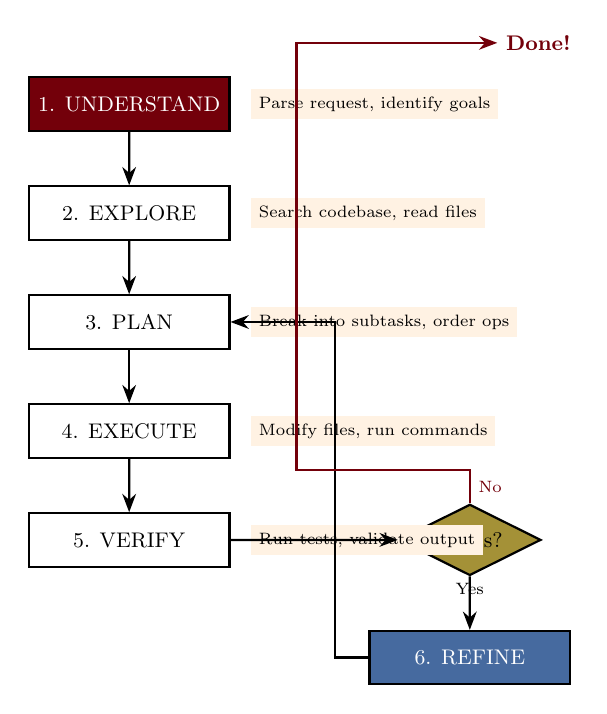
\begin{tikzpicture}[node distance=0.8cm and 0.5cm, scale=0.85, transform shape]
        % Nodes
        \node[process highlight] (understand) {1. UNDERSTAND};
        \node[process, below=of understand] (explore) {2. EXPLORE};
        \node[process, below=of explore] (plan) {3. PLAN};
        \node[process, below=of plan] (execute) {4. EXECUTE};
        \node[process, below=of execute] (verify) {5. VERIFY};
        \node[decision, right=2.5cm of verify] (issues) {Issues?};
        \node[process secondary, below=of issues] (refine) {6. REFINE};

        % Descriptions
        \node[label box, right=0.3cm of understand] {Parse request, identify goals};
        \node[label box, right=0.3cm of explore] {Search codebase, read files};
        \node[label box, right=0.3cm of plan] {Break into subtasks, order ops};
        \node[label box, right=0.3cm of execute] {Modify files, run commands};
        \node[label box, right=0.3cm of verify] {Run tests, validate output};

        % Arrows
        \draw[arrow] (understand) -- (explore);
        \draw[arrow] (explore) -- (plan);
        \draw[arrow] (plan) -- (execute);
        \draw[arrow] (execute) -- (verify);
        \draw[arrow] (verify) -- (issues);
        \draw[arrow] (issues) -- node[above, font=\scriptsize] {Yes} (refine);
        \draw[arrow] (refine.west) -- ++(-0.5,0) |- (plan.east);
        \draw[arrow garnet] (issues.north) |- node[right, font=\scriptsize, pos=0.25] {No} ++(0,0.5) -| ($(understand.north)+(2.5,0.5)$) -- ++(3,0) node[right, font=\small\bfseries, text=UofSCGarnet] {Done!};
    \end{tikzpicture}
    \end{center}

    \note{This loop is fundamental. Agents explore, understand, plan, then execute. Clear requests lead to efficient loops.}
\end{frame}

\begin{frame}{Core Capabilities at a Glance}
    \small
    \begin{tabular}{@{}lccl@{}}
        \toprule
        \textbf{Capability} & \textbf{Terminal} & \textbf{IDE} & \textbf{Description} \\
        \midrule
        Code Generation & \textcolor{UofSCHorseshoe}{\faCheck\faCheck} & \textcolor{UofSCHorseshoe}{\faCheck\faCheck} & Create files from scratch \\
        Multi-File Editing & \textcolor{UofSCHorseshoe}{\faCheck\faCheck} & \textcolor{UofSCHoneycomb}{\faCheck} & Modify multiple files at once \\
        Codebase Search & \textcolor{UofSCHorseshoe}{\faCheck\faCheck} & \textcolor{UofSCHorseshoe}{\faCheck\faCheck} & Find patterns, understand arch. \\
        Terminal Execution & \textcolor{UofSCHorseshoe}{\faCheck\faCheck} & \textcolor{UofSC50Black}{\faMinus} & Run commands in real-time \\
        Git Operations & \textcolor{UofSCHorseshoe}{\faCheck\faCheck} & \textcolor{UofSCHoneycomb}{\faCheck} & Commit, branch, PR automation \\
        Documentation & \textcolor{UofSCHorseshoe}{\faCheck\faCheck} & \textcolor{UofSCHoneycomb}{\faCheck} & Generate docs, comments \\
        Real-Time Feedback & \textcolor{UofSC50Black}{\faMinus} & \textcolor{UofSCHorseshoe}{\faCheck\faCheck} & Immediate suggestions \\
        Large Refactoring & \textcolor{UofSCHorseshoe}{\faCheck\faCheck} & \textcolor{UofSCHoneycomb}{\faCheck} & Project-wide code changes \\
        \bottomrule
    \end{tabular}

    \vspace{0.4cm}
    \textcolor{UofSCHorseshoe}{\faCheck\faCheck} = Excellent \quad
    \textcolor{UofSCHoneycomb}{\faCheck} = Good \quad
    \textcolor{UofSC50Black}{\faMinus} = Limited

    \note{Most productive developers use both---IDE plugin during development, terminal agent for larger tasks.}
\end{frame}

% ============================================================
% SECTION 2: CODE GENERATION & EDITING
% ============================================================
\section{Code Generation \& Editing}

\begin{frame}{Code Generation Fundamentals}
    \begin{center}
    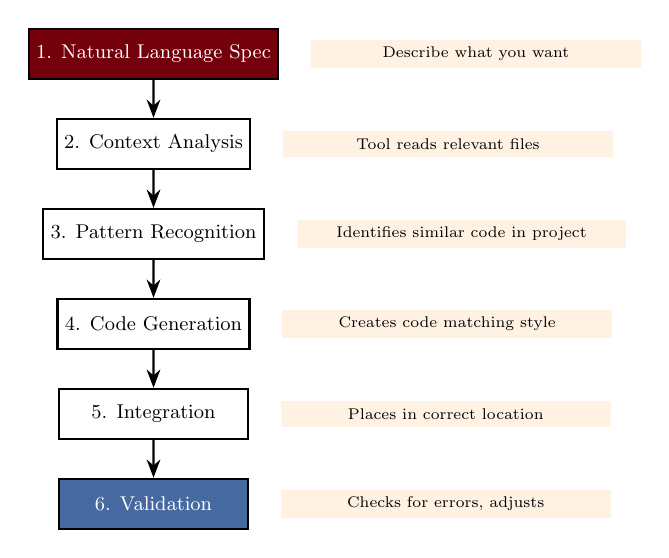
\begin{tikzpicture}[node distance=0.6cm, scale=0.8, transform shape]
        % Flow nodes
        \node[process highlight] (spec) {1. Natural Language Spec};
        \node[process, below=of spec] (context) {2. Context Analysis};
        \node[process, below=of context] (pattern) {3. Pattern Recognition};
        \node[process, below=of pattern] (gen) {4. Code Generation};
        \node[process, below=of gen] (int) {5. Integration};
        \node[process secondary, below=of int] (val) {6. Validation};

        % Arrows
        \draw[arrow] (spec) -- (context);
        \draw[arrow] (context) -- (pattern);
        \draw[arrow] (pattern) -- (gen);
        \draw[arrow] (gen) -- (int);
        \draw[arrow] (int) -- (val);

        % Side descriptions
        \node[label box, right=0.5cm of spec, text width=5cm] {Describe what you want};
        \node[label box, right=0.5cm of context, text width=5cm] {Tool reads relevant files};
        \node[label box, right=0.5cm of pattern, text width=5cm] {Identifies similar code in project};
        \node[label box, right=0.5cm of gen, text width=5cm] {Creates code matching style};
        \node[label box, right=0.5cm of int, text width=5cm] {Places in correct location};
        \node[label box, right=0.5cm of val, text width=5cm] {Checks for errors, adjusts};
    \end{tikzpicture}
    \end{center}

    \note{The agent learns your project's conventions automatically. Context is crucial for quality.}
\end{frame}

\begin{frame}[fragile]{Terminal Agent Example: Claude Code}
    \begin{lstlisting}[language=bash, title=Starting Claude Code]
# Start Claude Code with project context
claude code /workspace/api-project

# Request
> "Create a FastAPI endpoint that accepts POST requests
>  at /api/users with name and email, validates input
>  using Pydantic, stores in database, returns created
>  user with ID, includes error handling for duplicates"
    \end{lstlisting}

    \vspace{0.3cm}
    \textbf{Claude Code will automatically:}
    \begin{enumerate}
        \item Examine existing FastAPI route patterns
        \item Check Pydantic model structure
        \item Understand database schema from existing code
        \item Generate endpoint matching project style
        \item Add proper error handling and status codes
        \item Run validation to ensure integration
    \end{enumerate}

    \note{Claude Code runs directly in your terminal context, chaining operations automatically.}
\end{frame}

\begin{frame}[fragile]{Terminal Agent Example: Aider}
    \begin{columns}[T]
        \begin{column}{0.48\textwidth}
            \begin{lstlisting}[language=bash, title=Aider Setup]
# Install via pip
pip install aider-chat

# Start with specific files
aider src/main.py src/utils.py

# Interactive commands
aider> "Add JWT auth to login"
aider> "Refactor duplicated code"
aider> "Run tests, fix failures"
            \end{lstlisting}
        \end{column}
        \begin{column}{0.48\textwidth}
            \begin{lstlisting}[language=bash, title=Multi-File Refactoring]
aider> "Update User model to
>      add email_verified field"

# Aider:
# - Reads User model file
# - Identifies all usages
# - Updates model, migrations
# - Updates related code
# - Runs tests to verify
            \end{lstlisting}
        \end{column}
    \end{columns}

    \vspace{0.3cm}
    \textbf{Key Aider Features:}
    \begin{itemize}
        \item \texttt{/add src/file.py} -- Mark files for editing
        \item \texttt{/commit 'message'} -- Commit working changes
        \item Maintains context across multiple changes
    \end{itemize}

    \note{Aider is particularly good for conversational code editing with back-and-forth dialogue.}
\end{frame}

\begin{frame}[fragile]{IDE Agent Example: Cursor}
    \begin{center}
    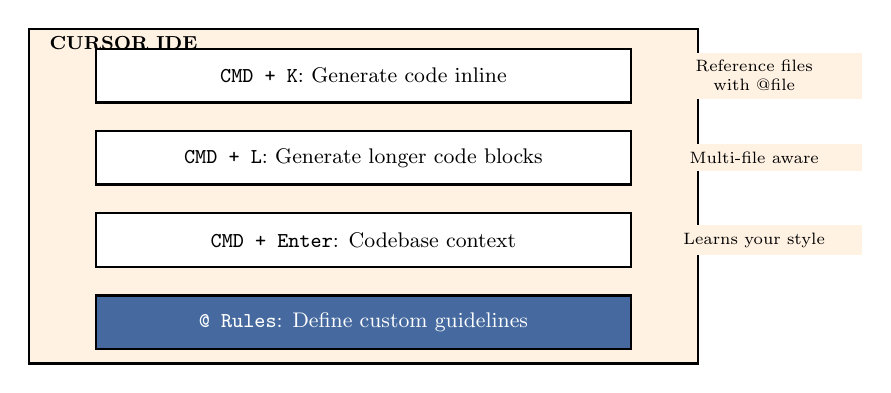
\begin{tikzpicture}[node distance=0.4cm, scale=0.85, transform shape]
        % IDE Window
        \node[rectangle, draw=UofSCBlack, thick, fill=UofSCSandstorm,
              minimum width=10cm, minimum height=5cm] (window) {};
        \node[anchor=north west, font=\footnotesize\bfseries] at (window.north west)
              {\hspace{0.2cm}CURSOR IDE};

        % Commands
        \node[process, minimum width=8cm, below=0.3cm of window.north] (cmd1)
              {\texttt{CMD + K}: Generate code inline};
        \node[process, minimum width=8cm, below=of cmd1] (cmd2)
              {\texttt{CMD + L}: Generate longer code blocks};
        \node[process, minimum width=8cm, below=of cmd2] (cmd3)
              {\texttt{CMD + Enter}: Codebase context};
        \node[process secondary, minimum width=8cm, below=of cmd3] (cmd4)
              {\texttt{@ Rules}: Define custom guidelines};

        % Descriptions
        \node[label box, right=0.2cm of cmd1.east, anchor=west, text width=3cm]
              {\scriptsize Reference files with @file};
        \node[label box, right=0.2cm of cmd2.east, anchor=west, text width=3cm]
              {\scriptsize Multi-file aware};
        \node[label box, right=0.2cm of cmd3.east, anchor=west, text width=3cm]
              {\scriptsize Learns your style};
    \end{tikzpicture}
    \end{center}

    \vspace{0.2cm}
    \textbf{Cursor learns your patterns:} imports, error handling, component preferences

    \note{Cursor bridges IDE and agent. The @ syntax references specific files for context.}
\end{frame}

\begin{frame}[fragile]{Multi-File Editing: The Power of Terminal Agents}
    \begin{columns}[T]
        \begin{column}{0.45\textwidth}
            \textbf{Traditional Approach:}
            \begin{enumerate}
                \item Update database schema
                \item Create migration
                \item Update ORM models
                \item Update all queries
                \item Update tests
                \item Update documentation
                \item Debug remaining issues
            \end{enumerate}
            \textcolor{UofSCRose}{\textit{Hours of work...}}
        \end{column}
        \begin{column}{0.52\textwidth}
            \textbf{With Terminal Agent:}
            \begin{lstlisting}[language=bash, basicstyle=\ttfamily\tiny]
aider> "Rename 'user_name' to 'username'
>       everywhere in the codebase.
>       Update migrations, models, queries,
>       tests, and API documentation."

# Agent output:
Found 47 occurrences in 6 files...
Updating files...
[1/6] migrations/001_rename.py
[2/6] models/user.py
[3/6] queries/user_queries.py
...
Running tests... All passing!
            \end{lstlisting}
            \textcolor{UofSCHorseshoe}{\textit{Minutes of work!}}
        \end{column}
    \end{columns}

    \note{This is what separates agentic tools---they understand semantic meaning and update dependent code accordingly.}
\end{frame}

\begin{frame}{Choosing the Right Tool}
    \small
    \begin{tabular}{@{}lll@{}}
        \toprule
        \textbf{Task} & \textbf{Best Tool} & \textbf{Why} \\
        \midrule
        Single function generation & Copilot, Cursor & Real-time, low friction \\
        Component/module generation & Cursor, Windsurf & Multiple file context \\
        Multi-file refactoring & Aider, Claude Code & Designed for this \\
        Learning new framework & Cursor, Copilot & Immediate feedback \\
        Understanding existing code & Copilot Chat, Claude Code & In-editor explanation \\
        Batch automation & Claude Code, Terminal agents & Scriptable, repeatable \\
        Architecture design & Claude Code, Windsurf Cascade & Reason about patterns \\
        \bottomrule
    \end{tabular}

    \vspace{0.4cm}
    \begin{alertblock}{Recommendation}
        Use IDE plugins during development for rapid iteration, then terminal agents for larger refactoring tasks. The tools complement each other.
    \end{alertblock}

    \note{Most productive developers use multiple tools in combination.}
\end{frame}

% ============================================================
% SECTION 3: FILE MANAGEMENT
% ============================================================
\section{File Management}

\begin{frame}{File Operations: Core Patterns}
    \begin{center}
    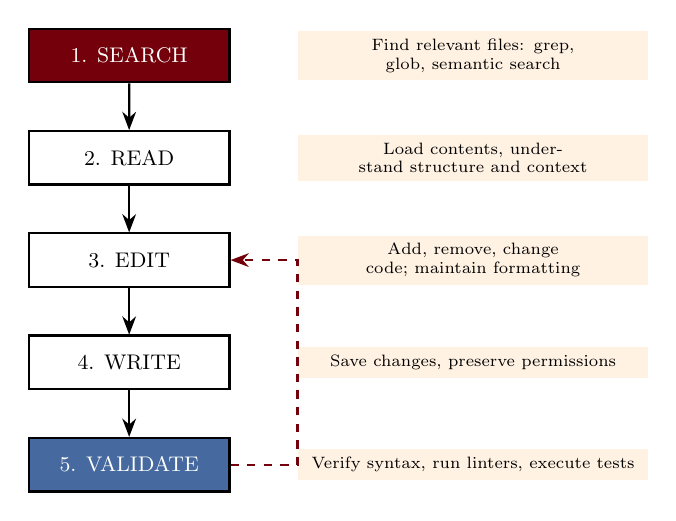
\begin{tikzpicture}[node distance=0.7cm, scale=0.85, transform shape]
        % Vertical flow
        \node[process highlight] (search) {1. SEARCH};
        \node[process, below=of search] (read) {2. READ};
        \node[process, below=of read] (edit) {3. EDIT};
        \node[process, below=of edit] (write) {4. WRITE};
        \node[process secondary, below=of write] (validate) {5. VALIDATE};

        % Descriptions on the right
        \node[label box, right=1cm of search, text width=5cm]
              {Find relevant files: grep, glob, semantic search};
        \node[label box, right=1cm of read, text width=5cm]
              {Load contents, understand structure and context};
        \node[label box, right=1cm of edit, text width=5cm]
              {Add, remove, change code; maintain formatting};
        \node[label box, right=1cm of write, text width=5cm]
              {Save changes, preserve permissions};
        \node[label box, right=1cm of validate, text width=5cm]
              {Verify syntax, run linters, execute tests};

        % Arrows
        \draw[arrow] (search) -- (read);
        \draw[arrow] (read) -- (edit);
        \draw[arrow] (edit) -- (write);
        \draw[arrow] (write) -- (validate);

        % Feedback loop
        \draw[arrow, dashed, color=UofSCGarnet] (validate.east) -- ++(1,0) |- (edit.east);
    \end{tikzpicture}
    \end{center}

    \note{The power is in the sequence---a student might ask to ``add authentication to all API endpoints'' and the agent handles the entire chain.}
\end{frame}

\begin{frame}[fragile]{Creating Files \& Project Structure}
    \begin{columns}[T]
        \begin{column}{0.48\textwidth}
            \textbf{Single File Creation:}
            \begin{lstlisting}[language=bash, basicstyle=\ttfamily\tiny]
claude code /workspace

"Create .env.example with all
required environment variables
and helpful comments"
            \end{lstlisting}

            \vspace{0.3cm}
            \textbf{Result:}
            \begin{lstlisting}[basicstyle=\ttfamily\tiny]
# .env.example
# Database Configuration
DATABASE_URL=postgresql://...
DATABASE_POOL_SIZE=10

# Authentication
JWT_SECRET=your-secret-key
JWT_EXPIRATION_HOURS=24
            \end{lstlisting}
        \end{column}
        \begin{column}{0.48\textwidth}
            \textbf{Full Project Structure:}
            \begin{lstlisting}[basicstyle=\ttfamily\tiny]
my_service/
|-- src/
|   |-- __init__.py
|   |-- main.py
|   |-- config.py
|   |-- users/
|   |   |-- models.py
|   |   |-- routes.py
|   |   +-- services.py
|   +-- database/
|       +-- connection.py
|-- tests/
|   |-- conftest.py
|   +-- test_users.py
|-- docker/
|   +-- Dockerfile
|-- requirements.txt
+-- .env.example
            \end{lstlisting}
        \end{column}
    \end{columns}

    \note{This capability is valuable for rapid project setup---focus on business logic, not scaffolding.}
\end{frame}

\begin{frame}[fragile]{Editing \& Modifying Files}
    \begin{columns}[T]
        \begin{column}{0.48\textwidth}
            \textbf{Before:}
            \begin{lstlisting}[language=python, basicstyle=\ttfamily\tiny]
def login(email, password):
    user = db.query(User).filter(
        User.email == email
    ).first()
    if not user:
        return None
    if user.password == password:
        return user
    return None
            \end{lstlisting}
        \end{column}
        \begin{column}{0.48\textwidth}
            \textbf{After (with agent edit):}
            \begin{lstlisting}[language=python, basicstyle=\ttfamily\tiny]
def login(email, password):
    user = db.query(User).filter(
        User.email == email
    ).first()
    if not user:
        raise ValueError("Invalid")
    if not verify_password(
        password, user.password_hash
    ):
        raise ValueError("Invalid")
    return user
            \end{lstlisting}
        \end{column}
    \end{columns}

    \vspace{0.3cm}
    \textbf{Key Capabilities:}
    \begin{itemize}
        \item Precise string replacement with context awareness
        \item Preserves indentation and formatting
        \item Maintains code style consistency
        \item Can handle multiple edits in single file atomically
    \end{itemize}

    \note{Unlike simple find-and-replace, agentic tools understand context and won't break files.}
\end{frame}

\begin{frame}[fragile]{Git Integration with File Operations}
    \begin{lstlisting}[language=bash, basicstyle=\ttfamily\small, title=Automatic Staging for Related Changes]
aider> "Add 'email_verified' field to User model.
>       Update migration, schema, tests, and API."

# Aider outputs:
Modified files:
  - models/user.py
  - database/migrations/20240115_add_email.py
  - schemas/user_schema.py
  - tests/test_user_model.py

Ready to commit? (y/n)
    \end{lstlisting}

    \vspace{0.3cm}
    \textbf{Benefits:}
    \begin{itemize}
        \item Logical grouping of related changes
        \item Atomic commits that make sense
        \item Clean, understandable project history
        \item Easy code review
    \end{itemize}

    \note{Git integration creates logical commits that group related changes together.}
\end{frame}

% ============================================================
% SECTION 4: WRITING & DOCUMENTATION
% ============================================================
\section{Writing \& Documentation}

\begin{frame}[fragile]{Documentation Generation from Code}
    \begin{columns}[T]
        \begin{column}{0.55\textwidth}
            \begin{lstlisting}[language=bash, basicstyle=\ttfamily\tiny]
claude code /workspace/project

"Generate comprehensive documentation
for the auth module in docs/AUTH.md.
Include:
- Overview of authentication system
- Flow diagrams (ASCII art)
- How to use each public function
- Security considerations
- Examples of common use cases"
            \end{lstlisting}
        \end{column}
        \begin{column}{0.42\textwidth}
            \textbf{Generated Output:}
            \begin{center}
            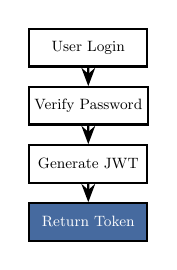
\begin{tikzpicture}[node distance=0.4cm, scale=0.6, transform shape]
                \node[process, minimum width=2.5cm] (login) {User Login};
                \node[process, below=of login, minimum width=2.5cm] (verify) {Verify Password};
                \node[process, below=of verify, minimum width=2.5cm] (jwt) {Generate JWT};
                \node[process secondary, below=of jwt, minimum width=2.5cm] (return) {Return Token};

                \draw[arrow] (login) -- (verify);
                \draw[arrow] (verify) -- (jwt);
                \draw[arrow] (jwt) -- (return);
            \end{tikzpicture}
            \end{center}
            \scriptsize Plus code examples, security notes, and usage patterns
        \end{column}
    \end{columns}

    \note{Documentation is often neglected. Agents can generate it first, encouraging self-documenting code.}
\end{frame}

\begin{frame}[fragile]{Inline Code Comments \& Docstrings}
    \begin{columns}[T]
        \begin{column}{0.48\textwidth}
            \textbf{Before:}
            \begin{lstlisting}[language=python, basicstyle=\ttfamily\tiny]
def authenticate_user(email, password):
    user = db.query(User).filter(
        User.email == email
    ).first()
    if not user:
        return None
    if verify_password(
        password, user.password_hash
    ):
        return user
    return None
            \end{lstlisting}
        \end{column}
        \begin{column}{0.48\textwidth}
            \textbf{After (with docstrings):}
            \begin{lstlisting}[language=python, basicstyle=\ttfamily\tiny]
def authenticate_user(
    email: str,
    password: str
) -> Optional[User]:
    """Authenticate user with
    email and password.

    Args:
        email: User's email.
        password: Plaintext password.

    Returns:
        User if successful, None
        otherwise.
    """
    # ... implementation
            \end{lstlisting}
        \end{column}
    \end{columns}

    \vspace{0.2cm}
    \begin{exampleblock}{Request}
        ``Add Google-style docstrings to all functions in models/user.py that don't have them.''
    \end{exampleblock}

    \note{Good comments are invaluable. Having an agent generate them ensures all code is documented.}
\end{frame}

\begin{frame}[fragile]{Type Hints \& Code Annotations}
    \begin{columns}[T]
        \begin{column}{0.48\textwidth}
            \textbf{Before:}
            \begin{lstlisting}[language=python, basicstyle=\ttfamily\tiny]
def get_user_by_email(email):
    return db.query(User).filter(
        User.email == email
    ).first()

def get_users_batch(user_ids):
    return db.query(User).filter(
        User.id.in_(user_ids)
    ).all()

def create_user(name, email, pwd):
    user = User(name=name, email=email)
    user.password_hash = hash(pwd)
    db.add(user)
    db.commit()
    return user
            \end{lstlisting}
        \end{column}
        \begin{column}{0.48\textwidth}
            \textbf{After:}
            \begin{lstlisting}[language=python, basicstyle=\ttfamily\tiny]
from typing import Optional, List
from models import User

def get_user_by_email(
    email: str
) -> Optional[User]:
    return db.query(User).filter(
        User.email == email
    ).first()

def get_users_batch(
    user_ids: List[int]
) -> List[User]:
    return db.query(User).filter(
        User.id.in_(user_ids)
    ).all()

def create_user(
    name: str, email: str, pwd: str
) -> User:
    # ... typed implementation
            \end{lstlisting}
        \end{column}
    \end{columns}

    \note{Type hints improve code quality and catch errors early. Agents add them automatically.}
\end{frame}

% ============================================================
% SECTION 5: CODEBASE RESEARCH & SEARCH
% ============================================================
\section{Codebase Research \& Search}

\begin{frame}{Semantic Code Search}
    \begin{columns}[T]
        \begin{column}{0.48\textwidth}
            \begin{alertblock}{Text Search (Traditional)}
                \texttt{grep "user\_id" *.py}
                \begin{itemize}
                    \item Finds all lines containing text
                    \item Lots of noise
                    \item Manual filtering required
                \end{itemize}
            \end{alertblock}
        \end{column}
        \begin{column}{0.48\textwidth}
            \begin{exampleblock}{Semantic Search (Agentic)}
                ``Find where user IDs are validated''
                \begin{itemize}
                    \item Agent understands \textit{validation} concept
                    \item Returns validation functions
                    \item Contextual results
                \end{itemize}
            \end{exampleblock}
        \end{column}
    \end{columns}

    \vspace{0.4cm}
    \textbf{Example Request:}
    ``Search the codebase for all database queries that touch the User table. Show direct queries, ORM queries, bulk operations, and identify any N+1 query problems.''

    \note{Semantic search gives you meaningful results, not just text matches.}
\end{frame}

\begin{frame}{Codebase Search Visualization}
    \begin{center}
    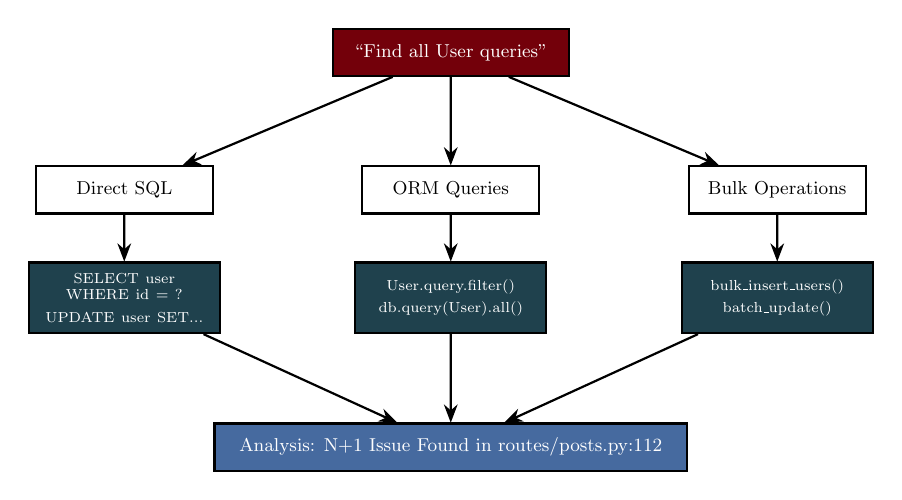
\begin{tikzpicture}[node distance=0.8cm and 1.5cm, scale=0.75, transform shape]
        % Central query
        \node[process highlight, minimum width=4cm] (query) {``Find all User queries''};

        % Search paths
        \node[process, below left=1.5cm and 2cm of query] (sql) {Direct SQL};
        \node[process, below=1.5cm of query] (orm) {ORM Queries};
        \node[process, below right=1.5cm and 2cm of query] (bulk) {Bulk Operations};

        % Results
        \node[process tertiary, below=of sql, text width=3cm, minimum height=1.2cm] (sql_r)
              {\scriptsize SELECT user WHERE id = ?\\UPDATE user SET...};
        \node[process tertiary, below=of orm, text width=3cm, minimum height=1.2cm] (orm_r)
              {\scriptsize User.query.filter()\\db.query(User).all()};
        \node[process tertiary, below=of bulk, text width=3cm, minimum height=1.2cm] (bulk_r)
              {\scriptsize bulk\_insert\_users()\\batch\_update()};

        % Analysis output
        \node[process secondary, below=1.5cm of orm_r, minimum width=8cm] (analysis)
              {Analysis: N+1 Issue Found in routes/posts.py:112};

        % Arrows
        \draw[arrow] (query) -- (sql);
        \draw[arrow] (query) -- (orm);
        \draw[arrow] (query) -- (bulk);
        \draw[arrow] (sql) -- (sql_r);
        \draw[arrow] (orm) -- (orm_r);
        \draw[arrow] (bulk) -- (bulk_r);
        \draw[arrow] (sql_r) -- (analysis);
        \draw[arrow] (orm_r) -- (analysis);
        \draw[arrow] (bulk_r) -- (analysis);
    \end{tikzpicture}
    \end{center}

    \note{Agent searches multiple dimensions and provides organized, actionable results.}
\end{frame}

\begin{frame}{Architecture Understanding}
    \begin{center}
    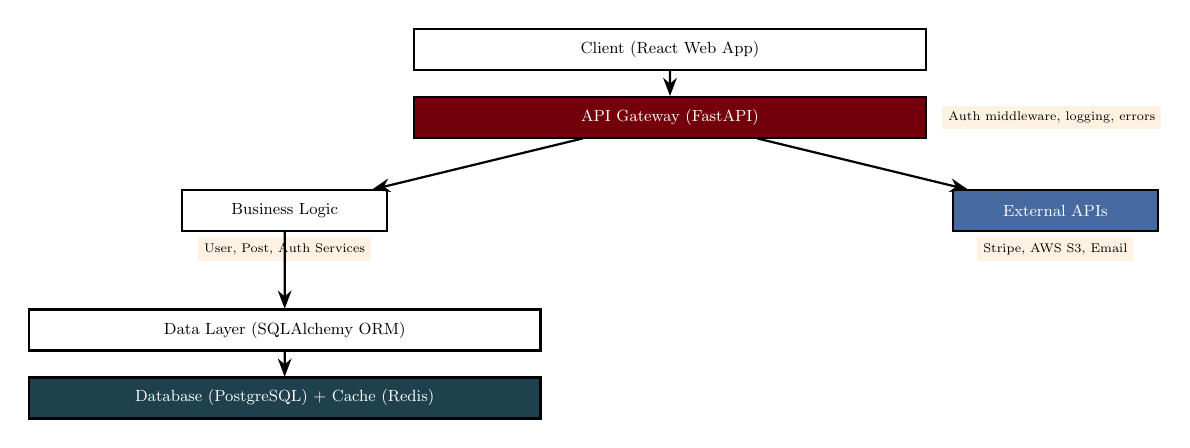
\begin{tikzpicture}[node distance=0.5cm, scale=0.65, transform shape]
        % Client layer
        \node[process, minimum width=10cm] (client) {Client (React Web App)};

        % API Gateway
        \node[process highlight, below=of client, minimum width=10cm] (api) {API Gateway (FastAPI)};
        \node[label box, right=0.3cm of api] {\scriptsize Auth middleware, logging, errors};

        % Services layer
        \node[process, below left=1cm and 0.5cm of api, minimum width=4cm] (business) {Business Logic};
        \node[process secondary, below right=1cm and 0.5cm of api, minimum width=4cm] (external) {External APIs};

        \node[label box, below=0.1cm of business] {\scriptsize User, Post, Auth Services};
        \node[label box, below=0.1cm of external] {\scriptsize Stripe, AWS S3, Email};

        % Data layer
        \node[process, below=1.5cm of business, minimum width=10cm] (data) {Data Layer (SQLAlchemy ORM)};

        % Database
        \node[process tertiary, below=of data, minimum width=10cm] (db) {Database (PostgreSQL) + Cache (Redis)};

        % Arrows
        \draw[arrow] (client) -- (api);
        \draw[arrow] (api) -- (business);
        \draw[arrow] (api) -- (external);
        \draw[arrow] (business) -- (data);
        \draw[arrow] (data) -- (db);
    \end{tikzpicture}
    \end{center}

    \vspace{0.2cm}
    \small Agent generates architecture diagrams, explains data flow, identifies patterns, and suggests improvements.

    \note{Understanding architecture accelerates onboarding and enables design discussions.}
\end{frame}

\begin{frame}[fragile]{Dependency Mapping}
    \begin{columns}[T]
        \begin{column}{0.48\textwidth}
            \textbf{Dependency Graph:}
            \begin{lstlisting}[basicstyle=\ttfamily\tiny]
main.py
|-- models/
|   |-- user.py
|   |   +-- database/connection.py
|   +-- post.py
|       |-- database/connection.py
|       +-- models/user.py (CIRCULAR!)
|
|-- routes/
|   |-- user_routes.py
|   |   |-- services/user_service.py
|   |   +-- models/user.py
|   +-- post_routes.py
|
+-- middleware/
    |-- auth_middleware.py
    +-- error_handler.py
            \end{lstlisting}
        \end{column}
        \begin{column}{0.48\textwidth}
            \textbf{Impact Analysis:}
            \begin{lstlisting}[language=bash, basicstyle=\ttfamily\tiny]
aider> "I want to add 'avatar_url'
>       to User model. Show impact."

# Direct imports needing updates:
# - services/user_service.py
# - routes/user_routes.py
# - tests/test_user.py

# Database impacts:
# - Need migration for new field
# - Update fixtures in tests

# API impacts:
# - User response schema
# - Documentation
            \end{lstlisting}
        \end{column}
    \end{columns}

    \vspace{0.2cm}
    \textbf{Benefit:} Understand refactoring impact before making changes!

    \note{Dependency mapping helps think systematically about change management.}
\end{frame}

\begin{frame}[fragile]{Finding Patterns \& Antipatterns}
    \begin{columns}[T]
        \begin{column}{0.48\textwidth}
            \textbf{Antipatterns Found:}

            \vspace{0.2cm}
            \textcolor{UofSCRose}{\faExclamationTriangle} \textbf{N+1 Query Problem}
            \begin{lstlisting}[language=python, basicstyle=\ttfamily\tiny]
# BAD: routes/posts.py:112
posts = db.query(Post).all()
for post in posts:
    author = db.query(User)...

# GOOD: Use eager loading
posts = db.query(Post).options(
    joinedload(Post.user)
).all()
            \end{lstlisting}

            \vspace{0.2cm}
            \textcolor{UofSCRose}{\faExclamationTriangle} \textbf{Bare Except}
            \begin{lstlisting}[language=python, basicstyle=\ttfamily\tiny]
# BAD: Catches everything!
except:
    return None

# GOOD: Specific exceptions
except RedisError:
    return None
            \end{lstlisting}
        \end{column}
        \begin{column}{0.48\textwidth}
            \textbf{Code Duplication Found:}

            \vspace{0.2cm}
            \textcolor{UofSCHoneycomb}{\faClone} \textbf{Type 1: Copy-Paste}
            \begin{itemize}
                \item Email validation in 2 files
                \item Extract to \texttt{validators.py}
            \end{itemize}

            \vspace{0.2cm}
            \textcolor{UofSCHoneycomb}{\faClone} \textbf{Type 2: Similar Logic}
            \begin{itemize}
                \item Error formatting in 3 middlewares
                \item Centralize in \texttt{error\_handler.py}
            \end{itemize}

            \vspace{0.2cm}
            \textcolor{UofSCHoneycomb}{\faClone} \textbf{Type 3: Validation}
            \begin{itemize}
                \item Password validation in 3 places
                \item Extract to single validator
            \end{itemize}
        \end{column}
    \end{columns}

    \note{Identifying patterns and antipatterns teaches best practices through your own code.}
\end{frame}

% ============================================================
% SECTION 6: ONLINE RESEARCH
% ============================================================
\section{Online Research}

\begin{frame}[fragile]{Web Search \& URL Fetching}
    \begin{columns}[T]
        \begin{column}{0.48\textwidth}
            \textbf{Direct Web Search:}
            \begin{lstlisting}[language=bash, basicstyle=\ttfamily\tiny]
claude code /workspace

"Search the web for:
1. JWT token best practices 2024
2. FastAPI security vulnerabilities
3. PostgreSQL vs MongoDB benchmarks
4. Python async optimization"

# Returns:
# - Current articles
# - Stack Overflow solutions
# - GitHub implementations
# - Performance benchmarks
            \end{lstlisting}
        \end{column}
        \begin{column}{0.48\textwidth}
            \textbf{URL Content Analysis:}
            \begin{lstlisting}[language=bash, basicstyle=\ttfamily\tiny]
"Visit fastapi.tiangolo.com/
advanced/middleware/ and tell me:
1. How middleware works
2. Key concepts
3. Code examples
4. Framework differences"

# Agent:
# - Fetches page
# - Extracts content
# - Analyzes examples
# - Summarizes concepts
            \end{lstlisting}
        \end{column}
    \end{columns}

    \vspace{0.3cm}
    \begin{block}{Research-Driven Development}
        ``We're considering switching from SQLAlchemy to SQLModel. Search for comparisons, adoption rates, known issues, and give me a recommendation.''
    \end{block}

    \note{Web search integration ensures students learn modern approaches, not decade-old patterns.}
\end{frame}

\begin{frame}[fragile]{Chaining Research Tasks}
    \begin{lstlisting}[language=bash, basicstyle=\ttfamily\small]
claude code /workspace

"Evaluate migrating from JWT to OAuth2. Please:
1. Search for security best practices comparing them
2. Fetch OAuth2 RFC and RFC 6750 standards
3. Analyze our current JWT implementation
4. Find 3 well-regarded OAuth2 open-source projects
5. Compare implementation complexity vs security
6. Estimate effort to migrate our 50+ endpoints
7. Make a recommendation with justification"
    \end{lstlisting}

    \vspace{0.3cm}
    \textbf{Result:} Comprehensive analysis that would take a human \textit{days} to compile, completed in minutes.

    \vspace{0.2cm}
    \textbf{Power of chaining:} Agent handles investigation upfront, then applies findings directly to your code.

    \note{Chaining bridges the gap between learning and implementation.}
\end{frame}

% ============================================================
% SECTION 7: GIT WORKFLOWS
% ============================================================
\section{Git Workflows}

\begin{frame}{Git Workflow with Agents}
    \begin{center}
    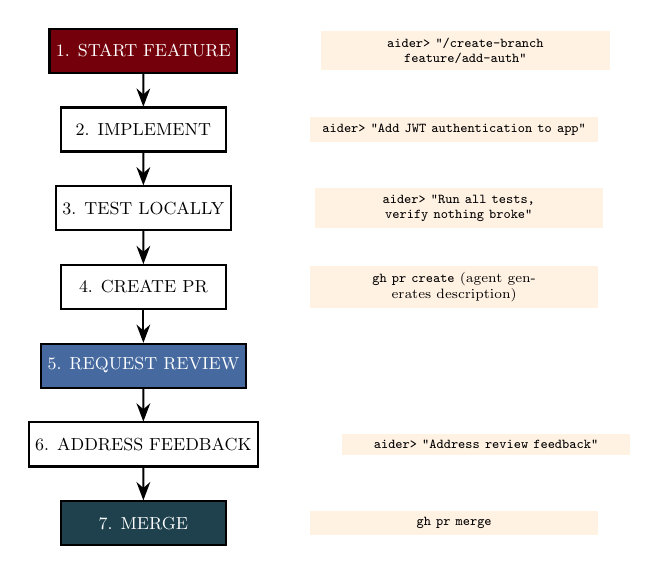
\begin{tikzpicture}[node distance=0.6cm, scale=0.7, transform shape]
        % Workflow steps
        \node[process highlight] (start) {1. START FEATURE};
        \node[process, below=of start] (implement) {2. IMPLEMENT};
        \node[process, below=of implement] (test) {3. TEST LOCALLY};
        \node[process, below=of test] (pr) {4. CREATE PR};
        \node[process secondary, below=of pr] (review) {5. REQUEST REVIEW};
        \node[process, below=of review] (feedback) {6. ADDRESS FEEDBACK};
        \node[process tertiary, below=of feedback] (merge) {7. MERGE};

        % Commands on the right
        \node[label box, right=1.5cm of start, text width=5cm]
              {\texttt{aider> "/create-branch feature/add-auth"}};
        \node[label box, right=1.5cm of implement, text width=5cm]
              {\texttt{aider> "Add JWT authentication to app"}};
        \node[label box, right=1.5cm of test, text width=5cm]
              {\texttt{aider> "Run all tests, verify nothing broke"}};
        \node[label box, right=1.5cm of pr, text width=5cm]
              {\texttt{gh pr create} (agent generates description)};
        \node[label box, right=1.5cm of feedback, text width=5cm]
              {\texttt{aider> "Address review feedback"}};
        \node[label box, right=1.5cm of merge, text width=5cm]
              {\texttt{gh pr merge}};

        % Arrows
        \draw[arrow] (start) -- (implement);
        \draw[arrow] (implement) -- (test);
        \draw[arrow] (test) -- (pr);
        \draw[arrow] (pr) -- (review);
        \draw[arrow] (review) -- (feedback);
        \draw[arrow] (feedback) -- (merge);
    \end{tikzpicture}
    \end{center}

    \note{This workflow combines all Git concepts. Agents automate mechanical work so humans can focus on meaningful review.}
\end{frame}

\begin{frame}[fragile]{Commit Management}
    \begin{columns}[T]
        \begin{column}{0.55\textwidth}
            \textbf{Atomic Commits:}
            \begin{lstlisting}[language=bash, basicstyle=\ttfamily\tiny]
aider> "Create 4 separate atomic commits:
>       1. Password hashing to Argon2
>       2. Email verification
>       3. Token generation refactor
>       4. Tests and documentation"

# Results:
feat(auth): migrate to Argon2
- Replace bcrypt for better security
- Update password validation

feat(auth): add email verification
- Require verification after signup
- Send emails via SMTP

refactor(auth): simplify token gen
- Extract token generation logic
- Improve error messages

test(auth): add tests and docs
- 12 new test cases
- Update API documentation
            \end{lstlisting}
        \end{column}
        \begin{column}{0.42\textwidth}
            \textbf{Conventional Commits:}

            \vspace{0.2cm}
            Format: \texttt{type(scope): subject}

            \vspace{0.3cm}
            \small
            \begin{tabular}{@{}ll@{}}
                \texttt{feat} & New feature \\
                \texttt{fix} & Bug fix \\
                \texttt{refactor} & Code refactoring \\
                \texttt{perf} & Performance \\
                \texttt{test} & Adding tests \\
                \texttt{docs} & Documentation \\
                \texttt{chore} & Build, deps \\
            \end{tabular}

            \vspace{0.3cm}
            \textbf{Agents automatically:}
            \begin{itemize}
                \item Analyze staged changes
                \item Generate meaningful messages
                \item Follow project conventions
            \end{itemize}
        \end{column}
    \end{columns}

    \note{Good commit messages are crucial. Agents teach message structure by example.}
\end{frame}

\begin{frame}[fragile]{Pull Request Creation}
    \begin{lstlisting}[language=bash, basicstyle=\ttfamily\small, title=Generated PR Description]
# Pull Request: Refactor Authentication System

## Description
Refactors auth system to improve security, maintainability,
and testability. All auth logic moved to dedicated service.

## Changes Made
- Created services/auth_service.py with centralized auth logic
- Migrated from bcrypt to Argon2 for password hashing
- Added email verification workflow

## Testing
- Added 15 new unit tests for auth service
- All existing tests still pass (127/127)

## Deployment Notes
- Requires new env vars: ARGON2_MEMORY, ARGON2_TIME
- Database migration required

Closes #234 - Improve authentication architecture
    \end{lstlisting}

    \note{PRs are how code gets reviewed. Agents help create comprehensive descriptions.}
\end{frame}

\begin{frame}[fragile]{Merge Conflict Resolution}
    \begin{columns}[T]
        \begin{column}{0.48\textwidth}
            \textbf{Conflict Analysis:}
            \begin{lstlisting}[basicstyle=\ttfamily\tiny]
File: src/services/user_service.py

Conflict 1 (Line 45):
Main branch:
  def get_user(user_id: int) -> User:

Feature branch:
  def get_user(user_id: int)
      -> Optional[User]:

Resolution: Use feature branch
(adds Optional type hint - improvement)

Conflict 2 (Line 67):
Main: Added caching decorator
Feature: Added logging decorator

Resolution: Keep both - combinable
  @cache_result
  @log_execution
  def search_users(query: str):
            \end{lstlisting}
        \end{column}
        \begin{column}{0.48\textwidth}
            \textbf{Request:}
            \begin{lstlisting}[language=bash, basicstyle=\ttfamily\small]
claude code /workspace

"Our feature branch has
conflicts with main. Please:
1. Identify conflicting files
2. Analyze root causes
3. Propose resolutions
4. Implement resolutions
5. Test to ensure nothing broke"
            \end{lstlisting}

            \vspace{0.3cm}
            \textbf{Agent provides:}
            \begin{itemize}
                \item Side-by-side comparison
                \item Intelligent merge proposals
                \item Automatic verification
            \end{itemize}
        \end{column}
    \end{columns}

    \note{Merge conflicts intimidate many students. Having an agent analyze them teaches what's happening.}
\end{frame}

% ============================================================
% CONCLUSION
% ============================================================
\section{Conclusion}

\begin{frame}{Key Takeaways}
    \begin{columns}[T]
        \begin{column}{0.48\textwidth}
            \begin{block}{Terminal Agents}
                Claude Code, Aider, GitHub Copilot CLI
                \begin{itemize}
                    \item Chain operations automatically
                    \item Best for multi-file refactoring
                    \item Scriptable and repeatable
                    \item CI/CD integration
                \end{itemize}
            \end{block}

            \begin{block}{Web Integration}
                \begin{itemize}
                    \item Search for solutions
                    \item Fetch documentation
                    \item Stay current with best practices
                \end{itemize}
            \end{block}
        \end{column}
        \begin{column}{0.48\textwidth}
            \begin{block}{IDE Plugins}
                Cursor, Windsurf, VS Code Copilot
                \begin{itemize}
                    \item Immediate suggestions
                    \item Less context-switching
                    \item Great for learning
                    \item Rapid prototyping
                \end{itemize}
            \end{block}

            \begin{block}{Git Integration}
                \begin{itemize}
                    \item Atomic commits
                    \item Meaningful messages
                    \item Branch management
                    \item PR automation
                \end{itemize}
            \end{block}
        \end{column}
    \end{columns}
\end{frame}

\begin{frame}{Next Steps}
    \begin{enumerate}
        \item \textbf{Choose your primary tool}
              \begin{itemize}
                  \item Recommend: Start with Cursor or Claude Code
              \end{itemize}
        \item \textbf{Practice simple tasks first}
              \begin{itemize}
                  \item File creation, reading, editing
              \end{itemize}
        \item \textbf{Graduate to multi-file operations}
              \begin{itemize}
                  \item Refactoring, testing
              \end{itemize}
        \item \textbf{Integrate into your workflow gradually}
        \item \textbf{Build custom workflows and automation}
    \end{enumerate}

    \vspace{0.5cm}
    \begin{exampleblock}{What's Next}
        Part 4 will cover: Advanced techniques, custom workflows, performance optimization, debugging with agentic tools, and building your own agentic workflows.
    \end{exampleblock}
\end{frame}

\begin{frame}{Quick Reference}
    \small
    \begin{columns}[T]
        \begin{column}{0.48\textwidth}
            \textbf{Terminal Agent Commands:}
            \begin{itemize}
                \item \texttt{claude code /path/to/project}
                \item \texttt{aider src/file1.py src/file2.py}
                \item \texttt{gh copilot suggest "..."}
                \item \texttt{gh copilot explain "..."}
            \end{itemize}
        \end{column}
        \begin{column}{0.48\textwidth}
            \textbf{Common Task Prompts:}
            \begin{itemize}
                \item ``Create a function that [desc]''
                \item ``Refactor [file] to [improvement]''
                \item ``Write tests for [module]''
                \item ``Help me debug [error]''
                \item ``Generate documentation for [module]''
            \end{itemize}
        \end{column}
    \end{columns}

    \vspace{0.5cm}
    \begin{center}
        \textbf{Resources:} Official documentation, YouTube tutorials, GitHub examples, community forums
    \end{center}
\end{frame}

\begin{frame}[plain]
    \begin{center}
        \vspace{2cm}
        {\Huge\textcolor{UofSCGarnet}{End of Part 3}}

        \vspace{1cm}
        {\Large Basic Usage}

        \vspace{1cm}
        {\large Questions?}

        \vspace{2cm}
        \textcolor{UofSC70Black}{\small Total Slides: 46 | Total Sections: 7}
    \end{center}
\end{frame}

\end{document}
